% 119-13(119쪽) — 곡선 y=-x^2+3x 와 x축으로 둘러싸인 도형을 직선 y=x 로 나눈 두 부분 S_1(곡선과 직선 사이) · S_2(직선·곡선과 x축 사이). 스캔 화질이 낮아 TikZ 로 다시 그림.
% 원문에 있는 것만: 눈금 3 · 라벨 O, x, y, y=-x^2+3x(지시선), y=x, S_1, S_2. 넓이 값은 넣지 않는다.
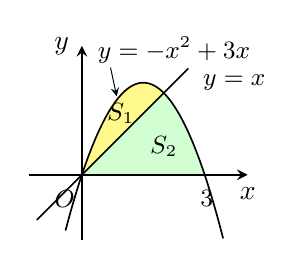
\begin{tikzpicture}[x=0.52cm, y=0.52cm, line width=0.5pt]
  % S_2 — x축 위 · 직선 y=x(0~2) 와 곡선(2~3) 아래
  \fill[green!18] (0,0) -- plot[domain=0:2, samples=40] (\x, {(\x)}) -- plot[domain=2:3, samples=50, smooth] (\x, {-(\x)*(\x)+3*(\x)}) -- cycle;
  % S_1 — 곡선과 직선 사이(0~2)
  \fill[yellow!45] plot[domain=0:2, samples=60, smooth] (\x, {-(\x)*(\x)+3*(\x)}) -- plot[domain=2:0, samples=40] (\x, {(\x)}) -- cycle;
  % 축
  \draw[->, >=stealth, line width=0.7pt] (-1.3,0) -- (4.05,0) node[below=1pt] {$x$};
  \draw[->, >=stealth, line width=0.7pt] (0,-1.6) -- (0,3.15) node[left=1pt] {$y$};
  % 곡선과 직선
  \draw[line width=0.6pt, domain=-0.4:3.45, samples=140, smooth] plot (\x, {-(\x)*(\x)+3*(\x)});
  \draw[line width=0.6pt] (-1.1,-1.1) -- (2.6,2.6);
  % 라벨(원문 자리 그대로)
  \node[below=2pt, font=\small] at (-0.42,0) {$\pt{O}$};
  \node[below=2pt, font=\small] at (3.05,0) {$3$};
  \node[font=\small] at (0.95,1.5) {$S_1$};
  \node[font=\small] at (2.0,0.7) {$S_2$};
  \node[anchor=west, font=\small] at (2.72,2.25) {$y=x$};
  \node[anchor=west, font=\small] at (0.15,3.05) {$y=-x^2+3x$};
  \draw[->, >=stealth, line width=0.35pt] (0.7,2.62) -- (0.85,1.92);
\end{tikzpicture}
